% !TEX root = ../thesis-example.tex
%
\chapter{Reinforcement Learning based methods}\label{sec:rl}
The idea of refining the sampling process of a diffusion model consists in correcting the sampling error related to the discretization of the backward SDE \ref{eq:backward_diffusion} or ODE. 
In section \ref*{sec:related:improve_generation}, we introduced \textit{rejection} sampling as a method to correct the sampling error. This method relies on using a trained discriminator to reject samples that are not close to the true distribution.
However, in high dimensions, the optimal acceptance probability of a sample becomes very small, which makes the rejection sampling method inefficient. We also would like to propose a method that is tailored for diffusion models, using the fact that the score network approximates the target distribution in different noise levels $t \in [0, T]$.
In the first section, we introduce restart sampling \citep{xu_restart_2023} as a \textit{boosting free} method to correct the sampling process. The method overall consists in improving the sampling process by solving the backward ODE \ref{eq:backward_diffusion}, renoising, and restarting the process for $K$ times. $K$ in this case is a hyperparameter that is manually tuned, thus raising the question of finding an optimal $K$ for a pre-trained diffusion model.
We propose to use Reinforcement Learning (RL) to instead dynamically noise / denoise the samples. We thus present briefly reinforcement learning in the second section, and formalize the problem for diffusion models in the third section. Experiments are currently ongoing for the end of the internship.




\section{Restart sampling}\label{sec:rl:sec1}
\subsection{Trade-off between speed and quality}
In order to sample from a diffusion model, the standard approach is to solve the backward ODE (Equation \ref{eq:backwatd_ode}) / SDE (Equation \ref{eq:backward_diffusion}) using numerical solvers, such as Heun's 2nd method and Euler-Maruyama's method \citep{kpj1992numerical}. The choice between reversing the ODE and the SDE is a trade-off between speed and quality : 
\begin{itemize}
    \item Sampling speed is evaluated for diffusion number by the number of function evaluations (NFE). That is, the number of calls to the score model $s_{\theta}$ during the sampling process. (Fast means low NFEs)
    \item Quality is commonly assessed by metrics depending on the data type. For image generation, the Fréchet Inception Distance (FID) \citep{heusel2017gans} is a common metric. (High quality means low FID)
\end{itemize}
As the sampling speed increases (low NFE), the sample quality generally deteriorates (high FID). This is explained by the discretization error caused by using a larger step size in numerical differential equation solvers.
As illustrated in figure \ref{fig:restart_sampling_nfe_quality}, ODE solvers are efficient in the small NFE regime, providing a decent quality with a large step size. They are outperformed by SDE solvers for smaller step sizes (high NFE) in terms of quality, and fail to improve when increasing the NFE.
\begin{figure}[htbp]
    \centering
    \begin{subfigure}{0.45\textwidth}
        \centering
        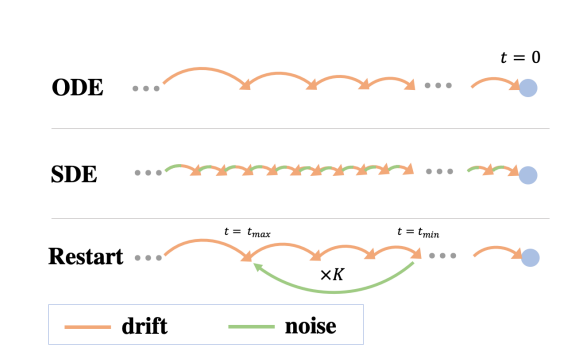
\includegraphics[width=\linewidth]{gfx/restart_sampling.png} % Left image
        \caption{Restart sampling method}
        \label{fig:restart_sampling}
    \end{subfigure}\hfill
    \begin{subfigure}{0.45\textwidth}
        \centering
        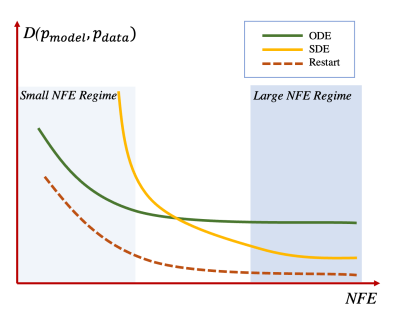
\includegraphics[width=\linewidth]{gfx/nfe_quality.png} % Right image
        \caption{Number of function evaluations (NFE) vs sampling quality}
        \label{fig:nfe_quality}
    \end{subfigure}
    \caption{Taken from \citep{xu_restart_2023}. \textbf{\ref*{fig:restart_sampling}} Illustration of restart sampling. \textbf{\ref*{fig:nfe_quality}} Sample quality vs NFE for different numerical solvers. ODE solvers (green) allow for a better quality than SDE solvers (yellow) in the small NFE regime, but plateau quickly in the large NFE regime.}
    \label{fig:restart_sampling_nfe_quality}
\end{figure}
\subsection{Sampling with ODE solvers vs SDE solvers}
In the small NFE regime, the effectiveness of ODEs can be explained by comparing the local error of the two methods. For a step size $\delta$, the Euler method for solving ODEs yields a local error of $O(\delta)^{2}$, while the Euler-Maruyama method for solving SDEs yields a local error of $O(\delta^{\frac{3}{2}})$ \citep{Dalalyan_2019}. 
In the large NFE regime, the step size $\delta$ becomes small thus the discrepancy between the two local errors becomes negligible. The main source of error thus becomes the \textit{approximation} error of the score model $s_{\theta}$. Intuitively, adding noise by solving the SDE corrects the approximation error. The absence of a noise term in the ODE solvers thus can be explained by the domination of the approximation error over the discretization error, that cannot be corrected via noise.
\citep{xu_restart_2023} provide a theorem that formalizes the behaviour difference between the two methods : 
\begin{theorem}\citep{xu_restart_2023}
Let $[t_{\min},t_{\max}] \subset [0,T] $, and let $\tilde{p}_{t}^{ODE}, \tilde{p}_{t}^{SDE}$ denote the distributions of simulating the ODE and SDE respectively, with the estimated score $s_{\theta}$. Assume for a given $B$
that $\forall t \in [t_{\min},t_{\max}], \|x_{t}\| \leq \frac{B}{2}$ for any $x_{t}$ in the support of $P_{t},\Tilde{P}_{t}^{ODE},\Tilde{P}_{t}^{SDE}$. Then we have the following upper bounds :
\begin{align}

    W_{1}(\tilde{p}_{t_{\min}}^{ODE},p_{t_{\min}}) &\leq B \cdot TV(\tilde{p}_{t_{\max}}^{ODE},p_{t_{\max}}) + O(\delta + \varepsilon_{\mathrm{approx}})(t_{\max}-t_{\min}) \\
    W_{1}(\tilde{p}_{t_{\min}}^{SDE},p_{t_{\min}}) &\leq \underbrace{(1-\lambda e^{-U})}_{\mathrm{contraction term}}\cdot B \cdot TV(\tilde{p}_{t_{\max}}^{SDE},p_{t_{\max}}) + O(\sqrt{\delta t_{\max}} + \varepsilon_{\mathrm{approx}})(t_{\max}-t_{\min})

\end{align}
where $W_{1}(.,.)$ denotes the 1-Wasserstein distance, $TV(.,.)$ denotes the total variation distance, $U = \frac{BL_{1}}{t_{\min}} + \frac{L_{1}^{2}t_{\max}^{2}}{t_{\min}^{2}}$, $\lambda < 1$ is a contraction factor, $L_{1}$ and $\varepsilon_{\mathrm{approx}}$ are uniform bounds on $\|ts_{\theta}(x,t)\|$ and the approximation error $\|ts_{\theta}(x,t) - t\nabla_{x} \log p_{t}(x)\|$ respectively.
\end{theorem}
Both right hand sides of the inequality feature two distinct terms in a sum. The first term denotes the \textit{contracted} error, i.e the initial errors
accumulated from both approximation and discretization errors during the simulation of the backward
process, up until time $t_{\max}$. The second term denotes the \textit{additional sampling} error. This term is essentially the same for both inequalities as $\delta$ gets small, but the contraction error is lowered by the term $U$ as the denoising process progresses, explaining the role of the noise in correcting the approximation error. 
This raises the following question : 
\textbf{Is there a sampling procedure that maintains the same discretization error as ODE solvers, while correcting the approximation error as SDE solvers do ?}

\subsection{Solving back and forth}
\citep{xu_2023_restart} propose \textit{restart sampling}, a sampling technique consisting in doing back and forth steps during the sampling process during a pre-defined time interval $[t_{\min},t_{\max}] \subset [0,T]$. As depicted in figure \ref{fig:restart_sampling}, a restart backward step consists in performing an ODE step from $t$ to $t-1$. A restart forward step consists in adding noise following the diffusion forward process (Equation \ref{eq:forward_diff}) from time $t_{\min}$ to time $t_{\max}$. This process is repeated $K$ times, and the final sample is the output of the last ODE backward step, from $t_{\min}$ to 0.
The authors provide the following upper bound on the 1-Wasserstein distance between the \textit{refined} distribution $Tilde{P}_{t_{\min}}^{\mathrm{restart}}$ and the target distribution $P_{t_{\min}}$:
\begin{equation}
    W_{1}(\Tilde{P}_{t_{\min}}^{\mathrm{restart}},P_{t_{\min}}) \leq B \cdot (1 - \lambda)^{K}TV(\Tilde{P}_{t_{\max}}^{\mathrm{restart}},P_{t_{\max}}) + (K+1) O(\delta + \varepsilon_{\mathrm{approx}})(t_{\max}-t_{\min})
\end{equation}
This inequality combines both advantages of ODE solvers (lower second term) and SDE solvers (approximation error contraction, exponential in $K$). 
However, this method introduces two additional degrees of freedom : the choice of the value of $K$ and the restart interval $[t_{\min},t_{\max}]$. This raises the following question : 
\textbf{Is it possible to dynamically noise / denoise the samples, without the need to manually tune $K$ ?}
We explore the option of using reinforcement learning as method to dynamically noise / denoise the samples, and present the formalization of the problem in the next section.
\section{Reinforcement Learning }\label{sec:rl:sec2}
\subsection{Background}
Reinforcement learning is a machine learning paradigm that stems from control theory. It essentially attempts to learn an optimal \textit{policy}, which is a probability distribution over actions given an observed state.
It is described by a markov decision process (MDP) tuple $(S, A, T, R, \gamma )$, where :
\begin{itemize}
    \item S is the set of states of the environment, that can either be continuous or discrete
    \item A is the set of actions that the agent can take
    \item T is the transition model such that $T(s'| s,a ) = P(S_{t+1} = s' | S_t = s , A_t = a)$
    \item R is the reward function that gives the reward r after taking action $a$ in state $s$
    \item $\gamma$ is the discount factor
\end{itemize}
A reinforcement learning \textit{agent} interacts with the environment during episodes. Given $s_{0} \sim \mu_{0}$, where $\mu_{0}$ is the distribution over initial states, the agent takes an action $a_{0}$ according to its policy $\pi_{\psi}$, and receives a reward $r_{0}$ and a new state $s_{1}$. The process is repeated until a terminal state is reached. The goal of the agent is to learn the optimal policy $\pi^{*}$ that maximizes the expected return :
\begin{equation}
    \mathcal{J}_{\mathrm{RL}}(\psi) = \mathbb{E}_{\pi_{\psi}}[\sum_{t=0}^{\infty} \gamma^{t}r_{t}]
\end{equation}
We denote by $\tau = (s_{0},a_{0},r_{0},s_{1},a_{1},r_{1},\ldots,s_{L})$ the trajectory of the agent by running an episode simulation in the environment.
The field of RL has gained a lot of attention in the past decade, with the advent of deep reinforcement learning involving deep neural networks \citep{mnih2013playingatarideepreinforcement}. It has been applied to several tasks, notably robotics \citep{gupta2019relaypolicylearningsolving}, protein synthesis \citep{jumper2021highly}, and famously for allowing the safe and aligned deployment of large language models through Reinforcement Learning from Human Feedback (RLHF) \citep{ouyang2022traininglanguagemodelsfollow}.
Several methods were developed to solve reinforcement learning, such as Q-learning, policy gradient methods, and actor-critic methods. Our work focuses on policy-gradient methods, and more specifically on the Proximal Policy Optimization (PPO) algorithm \citep{schulman2017proximal}. We present in the following section a modified version of the PPO algorithm that relies on $f-$divergences.
\subsection{Matching state visitation distributions}
The distribution over trajectories induced by the policy $\pi_{\psi}$ can be defined by the density : 
\begin{equation}
    p_{\psi}(\tau) = \mu_{0}(s_{0})\prod_{t=0}^{L-1} \pi_{\psi}(a_{t}|s_{t})p(s_{t+1}|s_{t},a_{t})
\end{equation}
Thus, the distribution over states induced by the policy $\pi_{\psi}$ can be defined by the density :
\begin{align}
    p_{\psi}(s) &= \frac{\int p_{\psi}(\tau)\eta_{\tau}(s) d\tau}{Z} \\
    &= \frac{\int \mu_{0}(s_{0})\prod_{t=0}^{L-1} \pi_{\psi}(a_{t}|s_{t})p(s_{t+1}|s_{t},a_{t})\eta_{\tau}(s)}{\int \int \mu_{0}(s_{0})\prod_{t=0}^{L-1} \pi_{\psi}(a_{t}|s_{t})p(s_{t+1}|s_{t},a_{t})\eta_{\tau}(s) d\tau ds } d\tau
\end{align}
with $\eta_{\tau}(s) = \sum_{s_{t} \in \tau } \delta(s - s_{t})$ the number of occurences of state $s$ in trajectory $\tau$.
As a result, the optimal policy similarly defines a disribution over state visitation, that we write as $P^{*}$ with density $p^{*}(s)$. This allows to formulate the following objective function :
\begin{equation}\label{eq:rl:learning_problem}
    \mathcal{J}_{\mathrm{RL}}(\psi) = D_{f}(p_{\theta},p^{*})
\end{equation}
\subsection{f-Policy gradient}
As explained in section \ref*{sec:rl:sec3}, this formulation allows to find an optimal policy without access to the reward function. This is crucial in our case since in the context of refining diffusion models, the only information we have are samples from the target distribution $P_{t}$ and the estimated score $s_{\theta}$.
Computing the $f-$divergence in equation \ref{eq:rl:learning_problem} is intractable, but \citep{agarwal_f-policy_2023} derive an expression for its gradient, in a similar flavor to the policy gradient theorem \citep{NIPS1999_464d828b} :
\begin{equation}
    \nabla  \mathcal{J}_{\mathrm{RL}}(\psi) =  \mathbb{E}_{P_{\psi}} \left[ \left( \sum_{t=1}^{L} \nabla_{\psi} \log \pi_{\psi}(a_{t}|s_{t})  \right) \left(\sum_{t=1}^{L}f'\left( \frac{p_{\psi}(s_{t})}{p_{*}(s_{t})} \right)   \right)   \right]
\end{equation}

In practice, computing this gradient is computationally intensive since it requires performing \textit{on policy} updates. That is, the policy used to interact with the environment is updated on the go. This is not feasible for complex environments, as learning quickly becomes sample inefficient.
In order to enforce off-policy learning, one idea \citep{agarwal_f-policy_2023} was to use importance sampling from another policy $\pi_{\psi'}$ to estimate the gradient. In order to provide a good estimation, the current policy $\pi_{\psi}$ and the estimating policy $\pi_{\psi'}$ should be close. This is enforced by the Proximal Policy Optimization (PPO) algorithm \citep{schulman2017proximal}, that constrains the policy update to a certain distance from the previous policy. This is done by clipping the ratio of the new policy to the old policy, and using the clipped ratio to compute the loss function. This leads to the following expression for the gradient of $\mathcal{J}_{\mathrm{RL}}(\psi)$ :
\begin{equation}
    \nabla  \mathcal{J}_{\mathrm{RL}}(\psi) =  \mathbb{E}_{(s_{t},a_{t}) \sim P_{ \psi'}} \left[  \min\left(r_{\psi}(s_{t},a_{t})F_{\psi'}(s_{t}),\mathrm{clip}\left(r_{\psi}(s_{t},a_{t}),1-\varepsilon,1+\varepsilon\right)F_{\psi'}(s_{t}) \right)  \right]
\end{equation}
where $r_{\psi}(s_{t},a_{t}) = \frac{\nabla_{\psi} \pi_{\psi}(a_{t}|s_{t})}{\pi_{\psi'}(a_{t}|s_{t})}$ is the importance sampling ratio, $F_{\psi'}(s_{t}) = \sum_{i=t}^{T} \gamma^{i} f'\left( \frac{p_{\psi'}(s_{i})}{p_{*}(s_{i})} \right)$, and $\varepsilon$ is a hyperparameter that controls the clipping of the ratio. Algorithm \ref*{alg:fpg} describes the generic training procedure for a given environment, and samples from the expert policy.
\begin{algorithm}
    \caption{f-PG}
    \label{alg:fpg}
    \begin{algorithmic}[1]
    \State Let $\pi_\psi$ be the policy, $B$ be a buffer, $\mathcal{S}$ the set of trajectories from the expert policy
    \For{$i = 1$ to $\text{num\_iter}$}
        \State $B \leftarrow []$
        \For{$j = 1$ to $\text{num\_traj\_per\_iter}$}
            \State Simulate trajectory $\tau$ using $\pi_\psi'$
            \State Train a discriminator $d_{\phi}$ to estimate the density ratio $\frac{p_{\psi'}(s)}{p_{*}(s)}$
            \State Store $f' \left( d_{\phi}(s) \right)$ for each $s$ in $\tau$
            \State $B \leftarrow B + \{\tau \}$
        \EndFor
        \For{$j = 1$ to $\text{num\_policy\_updates}$}
            \State $\theta \leftarrow \theta - \alpha \nabla_\psi J_{\mathrm{RL}}(\psi)$
        \EndFor
    \EndFor
    \end{algorithmic}
    \end{algorithm}
In the following section, we will devise a procedure to apply the f-PG algorithm to the problem of refining diffusion models.

\section{Application to diffusion models}\label{sec:rl:sec3}
\subsection{Formalizing the restart sampling problem as a reinforcement learning problem}
The sampling process of diffusion models can be seen as a trajectory in the state space of a reinforcement learning agent. We train an agent to decide whether an ODE denoising step can be done, or if noise should be added to the current sample. The goal of the agent is to minimize the $f-$divergence between the state visitation distribution of the current policy and the optimal policy: 
\begin{itemize}
    \item  The state space can be defined as the set of samples $x_{t}$ of the discretized denoising process. Note that the timestep $t$ refers to the noise level in the diffusion model. To make a difference with the time variable in the reinforcement learning context, we will refer to the RL timestep as $l$.
    \item The action space is discretized in two actions : perform one ODE denoising step to go from $x_{t}$ to $x_{t-1}$, or perform add noise to go from $x_{t}$ to $x_{t+1}$.
    \item The trajectory length is a fixed number of steps $L \geq T$
    \item The reward function is the $f-$divergence between the state visitation distribution of the current policy and the optimal policy.
    \item The samples from the expert (optimal) policy are the samples from the target distribution $P_{t}$. Each sample $x_{t}$ is obtained from samples $x_{0}$ from the initial distribution $P_{0}$ (dataset), diffused according to the forward diffusion equation (Equation \ref{eq:forward_diff}) up to time $t$.
\end{itemize}
Up to the current stage of the thesis, this approach is exploratory and we lacked time to provide theoretical guarantees on the validity of this method. The following section describes the training procedure, that we term as \textit{f-Restart sampling}.
\subsection{f-Restart sampling}
We train a neural network that represents the policy $\pi_{\psi}$ to output a probability distribution over the set of actions \{Noise,ODE step\}. We train the policy using the f-PG algorithm, with the discriminator $d_{\phi}$ estimating the density ratio $\frac{p_{\psi'}(s)}{p_{*}(s)}$. The training dataset $\mathcal{S}$ is composed of samples from the target distribution $P_{t}$, and the buffer $B$ is used to store the trajectories of the agent. The training process is done for a fixed number of iterations, with a fixed number of trajectories per iteration, and a fixed number of policy updates per iteration. The hyperparameters $\alpha$ and $\varepsilon$ are manually tuned. The training process is done in an off-policy manner, with the policy $\pi_{\psi'}$ used to generate the trajectories. The training procedure is summarized in Algorithm \ref{alg:frs}

\begin{algorithm}
    \caption{f-Restart sampling}
    \label{alg:frs}
    \begin{algorithmic}[1]
    \State Let $\pi_\psi$ be the policy, $B$ be a buffer, $\mathcal{S}$ denote the training dataset (samples from the target distribution)
    \For{$i = 1$ to $\text{num\_iter}$}
        \State $B \leftarrow []$
        \For{$j = 1$ to $\text{num\_traj\_per\_iter}$}
            \State sample $x_{T}^{0}$ from the prior distribution $\mathcal{N}(0,I_{d})$
            \State $x_{0} \leftarrow x_{T}^{0}$
            \State $t_{0} \leftarrow T$
            \For{$l = 1$ to $L$}
            \State Compute $\pi_{\psi}(a|x_{l})$ for each action $a \in \{ \text{Noise, ODE step} \}$ and choose the action with highest probability
            \If {action = Noise}
                \State $x_{l+1} \leftarrow  $ Noise $x_{t}^{l}$ following the forward diffusion process
                $t_{l+1} \leftarrow t_{l} + 1$
            \Else
                \State $x_{l+1} \leftarrow  $ Perform one step of ODE denoising
                $t_{l+1} \leftarrow t_{l} - 1$
            \EndIf
            \State Store $(x_{l},t_{l},a_{l},x_{l+1},t_{l+1})$ in $\tau$
            \EndFor
            \State Train a discriminator $d_{\phi}$ to estimate the density ratio $\frac{p_{\psi'}(s)}{p_{*}(s)}$
            \State Store $f' \left( d_{\phi}(s) \right)$ for each $s$ in $\tau$
            \State $B \leftarrow B + \{\tau \}$
        \EndFor
        \For{$j = 1$ to $\text{num\_policy\_updates}$}
            \State $\theta \leftarrow \theta - \alpha \nabla_\psi J_{\mathrm{RL}}(\psi)$
        \EndFor
    \EndFor
    \end{algorithmic}
    \end{algorithm}
During this procedure, the quantities $f' \left( d_{\phi}(s) \right)$ can be seen as a guiding signal for the sampling algorithm to correct the approximation error. If at a denoising timestep $t$ this signal is low, then the agent should add noise to the sample to correct the error, thus using the advantage of SDEs introduced in section \ref*{sec:rl:sec1}. A high signal encourages the agent to continue the ODE denoising process.

\subsection{Experiments and results}
In order to test our proposed method, we will use a toy example of a 2D DDPM diffusion model. The target distribution is a mixture of 10 isotropic Gaussians, and we consider a trained score network that is trained on a samples stemming from a subset of modes of the target distribution. We use $f(u) = u\logu$ for minimizing the KL divergence between the target distribution and the state visitation distribution.
The first problematic behaviour observed is that the policy $\pi_{\psi}$ favours the noising step over the ODE denoising step. After one training epoch, the probability of choosing the noise action is close to 1. This was expected as the distributions $P_{t}$ and $\Tilde{P}_{t}$ are very close when the noise step is high. A workaround to this issue is to use a \textit{shaping} technique, consisting in encouraging the agent in the initial stages of training to perform the ODE denoising step.
\\
\textbf{Time weighting :} In order to force the agent to perform the ODE denoising step at the inital stages of training, we add a denoising time weighting factor to the density ratio, which essentially puts more importance to the smaller values of $t$. In our experiments, we choose a weighting term $w(t)$ that is linearly decreasing with $t$.
The effect of this shaping method was quite strong, and induced the reverse problematic behaviour : the agent would perform the ODE denoising step at each timestep. A few tweakings on the weighting scheme $w(t)$ were attempted, but the results were not satisfactory.
Figure \ref{fig:shaping_effect} shows that the agent does not change its behaviour post training, resulting in not improving the sampling process. We conclude that our shaping method was not effective, and provide the following directions for future work :
\begin{figure}[htbp]
    \centering
    \begin{subfigure}{0.32\textwidth}
        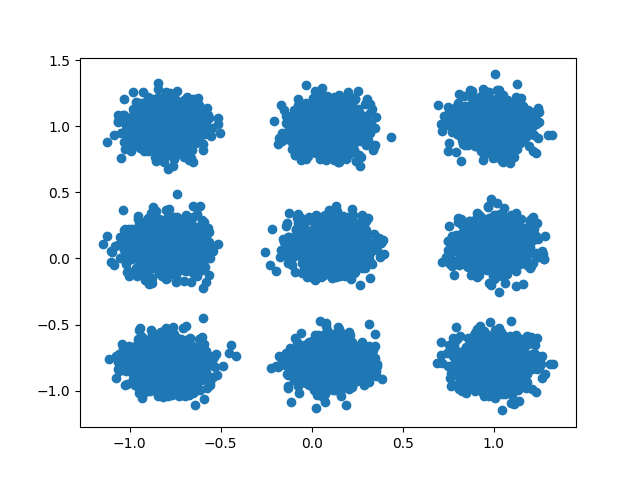
\includegraphics[width=\linewidth]{gfx/Real Data.png}
        \caption{Target distribution}
        \label{fig:target_samples}
    \end{subfigure}
    \hfill 
    \begin{subfigure}{0.32\textwidth}
        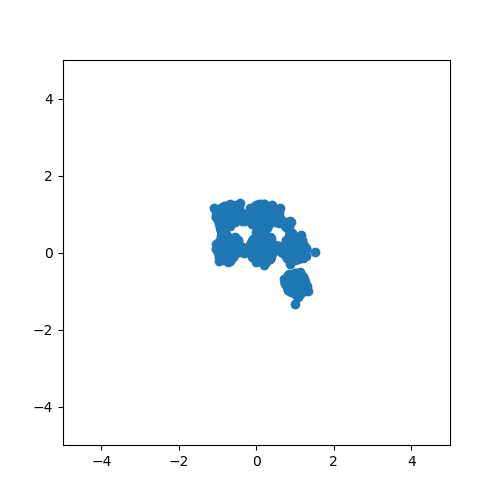
\includegraphics[width=\linewidth]{gfx/rl_before_train.png}
        \caption{Samples from $\Tilde{P}$ before training}
        \label{fig:pre_trained}
    \end{subfigure}
    \hfill 
    \begin{subfigure}{0.32\textwidth}
        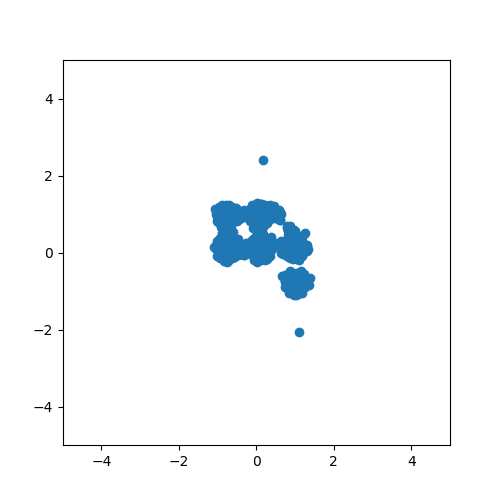
\includegraphics[width=\linewidth]{gfx/exponential_False_plots_rl_train_50.png}
        \caption{Samples from $\Tilde{P}$ after training}
        \label{fig:shaping}
    \end{subfigure}

    \caption{Reward shaping effect on the samples}
    \label{fig:shaping_effect}
\end{figure}
\begin{itemize}
    \item The optimality of the f-Restart sampling procedure was not proven. Further exploration on the theoretical aspect are needed to provide better insights for designing a training algorithm.
    \item Other shaping techniques should be considered to encourage the agent to perform the ODE denoising steps for high noise levels, but less frequently for low noise levels.
    \item Reinforcement learning relies on the Markov stationarity assumption, which might not be satisfied by our formulation of the state space. A more careful design of the state space should be considered.
\end{itemize}
\section{Conclusion}\label{sec:rl:conclusion}
In this chapter, we introduced the restart sampling method as a way to correct the sampling error of diffusion models. We then proposed to use reinforcement learning to dynamically noise / denoise the samples, and formalized the restart sampling procedure as a reinforcement learning problem. We presented the f-restart sampling algorithm, experimented on a toy example of a 2D diffusion model, and the results showed that our method was not effective. We provided directions for future work, notably on the theoretical aspect of the method, and on the design of the state space.

